%----------------------------------------------------------------------------------------
%   PACKAGES AND THEMES
%----------------------------------------------------------------------------------------

\documentclass{beamer}

\mode<presentation> {
\usetheme{Madrid}
\usecolortheme{crane}
}
\usepackage{listings}
\usepackage{graphicx} 
\usepackage{booktabs} 
\usepackage[italian]{babel}
\usepackage[utf8]{inputenc}
\usepackage[T1]{fontenc}
\usepackage{setspace}
\usepackage{listing}

%----------------------------------------------------------------------------------------
%   TITLE PAGE
%----------------------------------------------------------------------------------------

\title[Lambda in Java 8]{Lambda Expressions in Java 8: Uso e Tipaggio} 
\author[]{Mattia D'Autilia - 5765968 - mattia.dautilia@stud.unifi.it,\\ Alex Foglia - 6336805 - alex.foglia@stud.unifi.it}
\date{}

\begin{document}

%------------------------------------------------

\begin{frame}
	\frametitle{\textbf{Presentazione Seminario ATPL : 2017/2018}}
	\begin{center}
  		
\includegraphics[width=0.2\textwidth]{assets/logo-unifi.png}
  	\end{center}
	\titlepage 
\end{frame}

%------------------------------------------------

\begin{frame}
	\frametitle{\textbf{Indice presentazione}}
	\begin{enumerate}
	\begin{LARGE}
		\item
			\textbf{Java e Java 8}\\\
		\item
			\textbf{Lambda Expression Java 8}\\\
	\end{LARGE}
	\end{enumerate}
\end{frame}

%------------------------------------------------

\begin{frame}
	\frametitle{\textbf{1 : Java e Java 8}}
	\begin{center}
		\textbf{\Huge Java e Java 8}
	\end{center}
\end{frame}

%------------------------------------------------

\begin{frame}
	\frametitle{\textbf{1.1 : Java}}
	\begin{itemize}
		\item
			\textbf{Java} è un linguaggio di programmazione di alto livello, principalmente \textit{orientato agli oggetti}, ma accetta anche altri paradigmi come quello \textit{funzionale} ed è a \textit{tipizzazione statica}.\\\
		\item
			E' stato creato per soddisfare cinque obiettivi primari:
			\begin{enumerate}
				\item
					Essere "semplice e familiare";
				\item
					Essere "robusto e sicuro";
				\item
					Essere indipendente dalla piattaforma, da qui il detto \textit{"Write one, run everywhere"};
				\item
					Contenente strumenti e librerie per il networking;
				\item
					Essere progettato per eseguire codice da sorgenti remote in modo sicuro.
			\end{enumerate}
	\end{itemize}
\end{frame}

%------------------------------------------------

\begin{frame}
	\frametitle{\textbf{1.2 : Evoluzione di Java}}
		\begin{itemize}
			\item
				Quando Java nacque nel 1995, era un linguaggio molto semplice. Con il passare degli anni sono state introdotte gradualmente tante caratteristiche, diventando un linguaggio sempre più potente e completo,in particolare con la versione 5 e 7. Quello che però non era mai cambiato sino ad ora, era la coerenza d'essere un linguaggio orientato agli oggetti.
			\item 
				Negli ultimi anni però la scena della programmazione mondiale è cambiata. In particolare con l'avvento di processore multi-core nell'uso domestico, la \textit{programmazione funzionale} è stata rivalutata. Con linguaggi moderni come \textit{Scala e Groovy} è possibile scrivere algoritmi con un numero di righe nettamente inferiore, rispetto a quello che si poteva fare con Java, che qualcuno stava già definendo un linguaggio morto in quanto con le versioni 6 e 7 aveva solo modernizzato alcune librerie, estromettendo le tanto richieste \textit{Lambda Expression}.
		\end{itemize}
\end{frame}

%------------------------------------------------

\begin{frame}
	\frametitle{\textbf{1.3 : Java 8}}
	\begin{itemize}
		\item
			Con l'avvento di \textbf{Java 8} fu però apportata una vera e propria rivoluzione, la più innovativa in tutta la storia di Java. Con l'introduzione delle \textit{Espressioni Lambda} e la possibilità di \textit{referenziare i metodi}, la \textbf{filosofia funzionale}, fa il suo ingresso nella programmazione Java.
		\item
			Ora vedremo come affrontare la nuova sfida, che è quella di far convivere i due paradigmi, quello \textit{orientato agli oggetti} e quello \textit{funzionale}, in modo tale da ottenere il meglio della programmazione.				
	\end{itemize}
\end{frame}

%------------------------------------------------

\begin{frame}
	\frametitle{\textbf{2 : Lambda Expression in Java 8}}
	\begin{center}
		\textbf{\Huge Lambda Expression in Java8}
	\end{center}
\end{frame}

%------------------------------------------------

\begin{frame}
	\frametitle{\textbf{2.1 : Definizione}}
	\begin{itemize}
			\item
				Una \textbf{Lambda Expression} è detta:\\\
				\begin{itemize}
					\item
						\textbf{Funzione anonima} (in inglese \textbf{"anonymous function"}), in quanto si tratta proprio di una funzione, quindi non è un metodo appartenente a una classe e chiamato tramite un oggetto, ma è una funzione senza nome;
					\item \textbf{Chiusa} (in inglese \textbf{"closure"}), in quanto fa uso di variabili che non sono parametri e non sono variabili locali al blocco di codice che definisce l'espressione.\\\
				\end{itemize}
			\item
				Inoltre le \textbf{Lambda Expression} permettono:\\\
				\begin{itemize}
					\item
						di scrivere codice più semplice, leggibile e meno verboso;
					\item
						di adottare nuovi pattern di programmazione, basati sulle funzioni di \textbf{ordine superiore}.
				\end{itemize}				
	\end{itemize}
\end{frame}

%------------------------------------------------

\begin{frame}
	\frametitle{\textbf{2.2 : Sintassi}}
	\begin{itemize}
		\item
			In Java 8 la sintassi generale di una funzione è la seguente:\\\
			\begin{center}
				\Large ([lista di parametri])$\rightarrow$(espressione di ritorno)\\\
				\Large ([lista di parametri])$\rightarrow$\{blocco di codice come da prassi procedurale\}\\\
			\end{center}
		\item 
			Il vantaggio principale nell'uso di una \textit{Lambda Expression}, risiede nella sinteticità dell'espressione. In alcuni casi è possibile \textbf{omettere} :\\\
			\begin{enumerate}
				\item
					il \textbf{tipo dei parametri} quando non c'è possibilit\`a di errore;\\
				\item
					le parentesi tonde che circondano la lista dei parametri, nel caso quest'ultima fosse costituita da un unico elemento;\\
				\item
					la keyword \emph{return} quando esiste una singola espressione da valutare.		
			\end{enumerate}
	\end{itemize}	
\end{frame}

%------------------------------------------------

\begin{frame}
	\frametitle{\textbf{2.2 : Sintassi}}
	\begin{itemize}
		\item
			Abbiamo visto come una funzione viene definita in \textbf{Lambda Calcolo}. Facciamo l'esempio più semplice, la funzione identità:
			\begin{center}
				\Large$\lambda x.x$
			\end{center}
			\begin{itemize}
				\item
					\Large$\lambda$: rappresenta l'\textit{astrazione};
				\item
					la prima \Large $x$ : rappresenta la \textit{variabile di input};
				\item
					la seconda \Large $x$ : rappresenta il  \textit{corpo della funzione}.\\\
			\end{itemize}	
		\item
			Con queste regole di sintassi, tale funzione pu\`o essere scritta in uno qualsiasi dei seguenti modi:
			\begin{center}
				\Large$(x)\rightarrow(x)$
			\end{center}
			Oppure:
			\begin{center}
				\Large$x\rightarrow(x)$
			\end{center}
		\begin{center}
			\Large$x\rightarrow\{return\;x;\}$
		\end{center}											
	\end{itemize}
\end{frame}

%------------------------------------------------

\begin{frame}
	\frametitle{\textbf{2.3 : Quando usare le Lambda Expression}}
	\begin{itemize}
		\item
			Dovremmo usare le \textit{Lambda Expression,} quando il nostro obiettivo è quello di passare in maniera dinamica un certo algoritmo ad un altro metodo. Questo serve per eseguire l'algoritmo in un contesto definito dal metodo a cui stiamo passando l'algoritmo. \\\
		\item
			In generale, passare una \textit{Lambda Expression} a un metodo, significa delegare allo stesso la decisione sul \emph{se} e sul \emph{quando} valutare tale lambda.
	\end{itemize}
\end{frame}
%------------------------------------------------

\begin{frame}
	\frametitle{\textbf{2.3 : Quando usare le Lambda Expression}}
	\begin{itemize}
		\item
			In \textit{Java 8} \`e possibile usare una \textit{Lambda Expression} per:\\\
		\begin{itemize}
			\item
				\textbf{Assegnarla a una referenza} : trattarla come valore;\\\
			\item
				\textbf{Passarla come parametro} : parametrizzarla come comportamento;\\\
			\item
				\textbf{Ottenerla come risultato di una valutazione} : come un qualunque oggetto.
		\end{itemize}
	\end{itemize}
\end{frame}
%------------------------------------------------


\begin{frame}
	\frametitle{\textbf{2.4 : Funzioni di ordine superiore}}
	\begin{itemize}
		\item
			Nello studio del \textit{Lambda Calcolo}, abbiamo visto come le funzioni sono entità di prima classe: possono essere argomenti o anche risultato di una funzione.\\\
		\item
			Le \textbf{funzioni di ordine superiore} (in inglese \textbf{"higher order functions"}) sono funzioni che ammettono a loro volta funzioni come argomento e/o risultato. L'operatore matematico \emph{derivata} \`e un esempio di funzione d'ordine superiore.
	\end{itemize}
\end{frame}


%------------------------------------------------

\begin{frame}
	\frametitle{\textbf{2.4 : Funzioni di ordine superiore}}
	\begin{itemize}
		\item
			In Java le \textit{Lambda Expression} possono essere \textit{funzioni di ordine superiore}.\\\
		\item
			La possibilità di definire funzioni di ordine superiore rende Java 8 a tutti gli effetti un linguaggio che supporta anche il paradigma del \textit{Lambda Calcolo}.\\\	
		\item Vediamo alcuni esempi di implementazione in Java del \textbf{Lambda Calcolo}.
	\end{itemize}
\end{frame}

%----------------------------------------------------------------------------------------

\begin{frame}
	\frametitle{\textbf{2.5 : Lambda calcolo vs Lambda Expressions}}
	\begin{itemize}
		\item
			Funzione che riceve un intero \textit{x} e restituisce \textit{x+1}:\\\
		\begin{itemize}
			\item 
				\textbf{Lambda calcolo}:\\\
				\begin{center} 
					$\lambda x.x+1$ 
				\end{center}
			\item 
				\textbf{Java}:\\\
				\begin{figure}
					\centering
					
\includegraphics[width=0.3\linewidth]{image/identity.png}
					\label{fig:identity}
				\end{figure}
		\end{itemize}
	\end{itemize}
\end{frame}

%----------------------------------------------------------------------------------------

\begin{frame}
	\frametitle{\textbf{2.5 : Lambda calcolo vs Lambda Expressions}}
	\begin{itemize}
		\item
			La \textbf{curryficazione} di funzione binaria utilizzando \textit{higher-order-functions}:\\\
			\begin{itemize}
				\item 
					\textbf{Lambda calcolo}:
						\[
							\lambda xy.x+y
						\]
						\[
							\lambda x.\lambda y.x+y
						\]\\\
				\item 
					\textbf{Java}:
					\begin{figure}
						\centering
						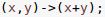
\includegraphics[width=0.3\linewidth]{image/double.png}
						\label{fig:double}
					\end{figure}
					\begin{figure}
						\centering
						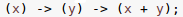
\includegraphics[width=0.4\linewidth]{image/curry.png}
						\label{fig:curry}
					\end{figure}
			\end{itemize}
	\end{itemize}
\end{frame}

%----------------------------------------------------------------------------------------

\begin{frame}
	\frametitle{\textbf{2.5 : Lambda calcolo vs Lambda Expressions}}
	\begin{itemize}
		\item
			\textbf{Booleani}:\\\
			\begin{itemize}
				\item 
					\textbf{Lambda calcolo}:\\\
						\[
							True = \lambda x.\lambda y.x
						\]
						\[
							False = \lambda x.\lambda y.y
						\]\\\
				\item 
					\textbf{Java}:\\\
					\begin{figure}
						\centering
						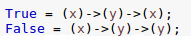
\includegraphics[width=0.4\linewidth]{image/booleani.png}
						\label{fig:identity}
					\end{figure}
			\end{itemize}	
	\end{itemize}
\end{frame}

%----------------------------------------------------------------------------------------

\begin{frame}
	\frametitle{\textbf{2.5 : Lambda calcolo vs Lambda Expressions}}
	\begin{itemize}
		\item
			\textbf{Ricorsione}:\\\
			\begin{itemize}
				\item 
					Supponiamo di voler scrivere una lambda per calcolare il \textit{fattoriale} di un numero intero:\\\
					\begin{itemize}
						\item 
							In \textbf{Lambda Calcolo}, sarebbe:\\\ 
								\[
							 		let \quad Fact = \lambda n. if(n=0) \quad 1 \quad else \quad n*Fact(n-1)
								\]\\\				 
						\item 
							Che in \textbf{Java} sarebbe:
								\begin{figure}
									\centering
									
\includegraphics[width=0.5\linewidth]{image/factwrong.png}
									\label{fig:identity}
								\end{figure}
					\end{itemize}
				\item 
					Come sappiamo dal \textit{Lambda Calcolo}, questa espressione non è corretta, poiché la lambda, essendo \textit{funzione anonima}, non può sapere di chiamarsi \textit{Fact}.
			\end{itemize}
	\end{itemize}
\end{frame}

%----------------------------------------------------------------------------------------

\begin{frame}
	\frametitle{\textbf{2.5 : Lambda calcolo vs Lambda Expressions}}
	\begin{itemize}
		\item
			\textbf{Ricorsione - Continuo}:\\\
			\begin{itemize}
				\item 
					Possiamo quindi implementare un \textbf{Combinatore di Punto Fisso}.\\\
				\begin{itemize}
					\item
						Nel \textbf{Lambda Calcolo}, un noto \textit{Combinatore di Punto Fisso} è il seguente:\\\
							\[
								fix = \lambda f.(\lambda x.f(xxy))(\lambda x.f(\lambda y.xxy))
							\]
					\item
						In \textbf{Java} possiamo definire suddetto \textit{combinatore} come segue:\\\
							\begin{figure}
								\centering
								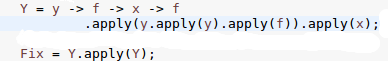
\includegraphics[width=0.8\linewidth]{image/fix.png}
								\label{fig:identity}
							\end{figure}
				\end{itemize}
			\end{itemize}
	\end{itemize}
\end{frame}

%----------------------------------------------------------------------------------------

\begin{frame}
	\frametitle{\textbf{2.5 : Lambda calcolo vs Lambda Expressions}}
	\begin{itemize}
		\item
			\textbf{Ricorsione - Continuo}:\\\
			\begin{itemize}
				\item 
					Applicando il \textit{Combinatore di Punto Fisso} al \textit{fattoriale}, otteniamo quindi:\\\
					\begin{itemize}
						\item 
							In \textbf{Lambda Calcolo}:\\\
								\[
									let \quad G = fix \quad Fact
								\]\\\
						\item 
							In \textbf{Java}:\\\
								\begin{figure}
									\centering
									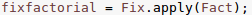
\includegraphics[width=0.8\linewidth]{image/factok.png}
									\label{fig:identity}
								\end{figure}
					\end{itemize}
			\end{itemize}
	\end{itemize}
\end{frame}

%----------------------------------------------------------------------------------------

\begin{frame}
\frametitle{\textbf{2.6 : Tipaggio}}
\begin{itemize}
	\item Finora abbiamo trattato le Lambda senza specificare il modo in cui queste possono essere assegnate a una variabile (o usarle come parametro di un metodo).
	\item Abbiamo inoltre visto come alcune lambda expressions possono essere valutate chiamando il metodo \emph{apply()}
	\item Entriamo nel dettaglio
\end{itemize}
\end{frame}

%----------------------------------------------------------------------------------------

\begin{frame}
\frametitle{\textbf{2.6 : Tipaggio}}
\begin{itemize}
	\item Java \`e un linguaggio \emph{strongly typed}
	\item Ogni sotto-espressione di qualsiasi espressione deve essere \emph{ben tipata}
	\item Quindi il tipo di una lambda deve essere coerente con il suo \emph{tipo atteso}
\end{itemize}
\end{frame}

%----------------------------------------------------------------------------------------

\begin{frame}[fragile]
\frametitle{\textbf{2.6 : Tipaggio}}
\begin{itemize}
	\item Per esempio, se scriviamo:
	\begin{figure}
		\centering
		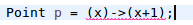
\includegraphics[width=0.3\linewidth]{image/target.png}
		\label{fig:target}
	\end{figure}
	\item Otteniamo il seguente errore:
	\begin{lstlisting}
	The target type of this expression
	must be a functional interface
	\end{lstlisting}
	\item Perchè la referenza a una lambda deve essere un' \emph{Interfaccia Funzionale}
\end{itemize}
\end{frame}

%----------------------------------------------------------------------------------------

\begin{frame}
\frametitle{\textbf{2.6.1 : Interfaccie funzionali}}
\begin{itemize}
	\item Una qualunque interfaccia è funzionale se e solo se contiene esattamente un solo metodo astratto.
	\item La signatura di questo metodo descrive il \emph{TIPO} di una Lambda Expression
	\item Quindi il tipo di una Lambda Expression \`e un' interfaccia funzionale
	\item Una lambda è come se fosse un'istanza di una classe concreta che implementa l'interfaccia funzionale
\end{itemize}
\end{frame}

%----------------------------------------------------------------------------------------

\begin{frame}
\frametitle{\textbf{2.6.1 : Interfaccie funzionali}}
\begin{itemize}
	\item Adesso possiamo capire l'errore precedente:
	\begin{figure}
		\centering
		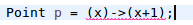
\includegraphics[width=0.3\linewidth]{image/target.png}
		\label{fig:target}
	\end{figure}
	\item In questo caso il type checker da errore in quanto la lambda expression non matcha con la signatura di alcun metodo astratto di un'interfaccia funzionale.
\end{itemize}
\end{frame}

%----------------------------------------------------------------------------------------

\begin{frame}
\frametitle{\textbf{2.6.2 : Typing}}
\begin{itemize}
	\item Il tipo di una lambda viene inferito rispetto alla sua interfaccia funzionale
	\item Il type-checker pu\`o stabilire se una lambda \`e ben tipata quando quest'ultima matcha con la signatura del metodo astratto
	\item Vediamo un esempio
\end{itemize}
\end{frame}

%----------------------------------------------------------------------------------------

\begin{frame}[fragile]
\frametitle{\textbf{2.6.2 : Typing}}
\begin{itemize}
	\item Java mette a disposizione la seguente interfaccia funzionale:
	\begin{lstlisting}[language=Java]
	public interface Function<T,S> {
		public S apply(T s);
	}
	\end{lstlisting}
	\item Quindi come fa il type checker a stabilire se la seguente lambda è ben tipata?
	\begin{lstlisting}[language=Java]
	Function<Integer,Boolean> fun=x->(x>=0);
	\end{lstlisting}
\end{itemize}
\end{frame}

%----------------------------------------------------------------------------------------

\begin{frame}[fragile]
\frametitle{\textbf{2.6.2 : Typing}}
\begin{itemize}
	\item Controlla se, assunto il parametro x di tipo Integer, il body della lambda è un Boolean.
	\item Dunque, assunto che x è un intero, è vero che $x>=0$ è un booleano? Si, la lambda è ben tipata.
\end{itemize}
\end{frame}

%----------------------------------------------------------------------------------------

\end{document}
              